% % % % % % % % % % % % % % % % % % % % % % % % % % % % % % % % % % % % % % % % % % % %
%                                                                                     %
% Short Sectioned Assignment LaTeX Template Version 1.0 (5/5/12)                      %
% This template has been downloaded from: http://www.LaTeXTemplates.com               %
%                                                                                     %
% Original author:  Frits Wenneker (http://www.howtotex.com)                          %
%                                                                                     %
% Modified by: Fco Javier Sueza Rodríguez (fcosueza@disroot.org)                      %
%                                                                                     %
% Changes:                                                                            %
%	    - Custom Chapters, Sections and Subsections (titlesec package)                %
%           - Document type scrbook (oneside)                                         %
%           - Use babel-lang-spanish package and marvosym                             %
%           - Use hyperref, enumitem, tcolorbox and glossaries packages               %
%           - Use Time New Roman (mathptmx), Helvetic and Courier fonts               %
%                                                                                     %
% License: CC BY-NC-SA 3.0 (http://creativecommons.org/licenses/by-nc-sa/3.0/)        %
%                                                                                     %
% % % % % % % % % % % % % % % % % % % % % % % % % % % % % % % % % % % % % % % % % % % %

%-----------------------------------------------%
%	              Packages                  %
%-----------------------------------------------%

\documentclass[paper=a4, fontsize=11pt, oneside]{scrbook}

% ---- Text Input/Output ----- %

\usepackage[T1]{fontenc}
\usepackage[utf8]{inputenc}
\usepackage{mathptmx}
\usepackage[scaled=.92]{helvet}
\usepackage{courier}
\usepackage[indent=12pt]{parskip}

\usepackage{geometry}
\geometry{verbose,tmargin=3cm,bmargin=3cm,lmargin=2.6cm,rmargin=2.6cm}

% ---- Language ----- %

\usepackage[spanish]{babel}
\usepackage{marvosym}

% ---- Another packages ---- %

\usepackage{amsmath,amsfonts,amsthm}
\usepackage{graphics,graphicx}
\usepackage{titlesec}
\usepackage{fancyhdr}
\usepackage{tcolorbox}
\usepackage{hyperref}
\usepackage{enumitem}
\usepackage[automake]{glossaries}

%--------------------------------------------------------------------%
%                      Customizing Document                          %
%--------------------------------------------------------------------%


% ----------- Custom Chapters, Sections and Subsections -------------- %

\titleformat{\chapter}[display]
			{\bfseries\Huge}
			{Tema \ \thechapter} {0.5ex}
			{\vspace{1ex}\centering}

\titleformat{\section}[hang]
			{\bfseries\Large}
			{\thesection}{0.5em}{}

\titleformat{\subsection}[hang]
			{\bfseries\large}
			{\thesubsection}{0.5em}{}

\titleformat{\subsubsection}[hang]
			{\bfseries\large}
			{\thesubsubsection}{0.5em}{}

\hypersetup{
    colorlinks=true,
    linkcolor=black,
    urlcolor=magenta
}

% ------------------- Custom heaaders and footers ------------------- %

\pagestyle{fancyplain}

\fancyhead[]{}
\fancyfoot[L]{}
\fancyfoot[C]{}
\fancyfoot[R]{\thepage}

\renewcommand{\headrulewidth}{0pt} % Remove header underlines
\renewcommand{\footrulewidth}{0pt} % Remove footer underlines

\setlength{\headheight}{13.6pt} % Customize the height of the header

% --------- Numbering equations, figures and tables ----------------- %

\numberwithin{equation}{section} % Number equations within sections
\numberwithin{figure}{section} % Number figures within sections
\numberwithin{table}{section} % Number tables within sections

% ------------------------ New Commands ----------------------------- %

\newcommand{\horrule}[1]{\rule{\linewidth}{#1}} % Create horizontal rule command


%----------------------------------------------------------------------------------------
%	TÍTULO Y DATOS DEL ALUMNO
%----------------------------------------------------------------------------------------

\title{
\normalfont \normalsize
\huge \textbf{Instalación del ERP Odoo}
}
\author{Francisco Javier Sueza Rodríguez}
\date{\normalsize\today}

%----------------------------------------------------------------------------------------
%                                     DOCUMENTO
%----------------------------------------------------------------------------------------
\begin{document}

\maketitle

\vspace{2ex}

\begin{center}
    \begin{tabular}{l l}
        \textbf{Centro}: & IES Aguadulce \\
        \textbf{Ciclo Formativo}: & Desarrollo Aplicaciones Web (Distancia)\\
        \textbf{Asignatura}: & Lenguajes de Marcas y Sistemas de Gestión de la Información\\
        \textbf{Tema}: & Tema 1 - Aspectos Básicos de los LM y SGI \\
    \end{tabular}
\end{center}

\vspace{10ex}

\section{Descripción}
En este ejercicio se va a realizar la instalación de un sistema ERP, en concreto de \textbf{Odoo}. Posteriormente, se van a instalar varios módulos, configurando y añadiendo diferente información a cada uno de ellos. La lista de tareas completa es la siguientes:

\begin{enumerate}
    \item \textbf{Instalación y configuración de Odoo}: instalar Odoo ya sea mediante una máquina virtual o usando la versión web.
    \item \textbf{Usuarios}: creación de dos usuarios, uno con datos personales y otro con datos del profesor/a.
    \item \textbf{Informe de productos}: instalar el módulo ``inventario'', crea tres paquetes diferentes y genera un informe de productos creados. Explora el informe en una hoja de cálculo.
    \item \textbf{Petición de mantenimiento}: instala el módulo ``Mantenimiento'' y crea dos peticiones de mantenimiento, una que este en estado ``En Proceso'' y otra en estado ``Reparado''.
\end{enumerate}

\section{Instalación de Odoo}
En primer lugar vamos a instalar Odoo. Nosotros hemos elegido realizar una instalación mediante \textbf{máquina virtual} usando \textbf{VirtualBox}. La instalación de la máquina virtual no entra dentro de este documento, así que supondremos que ya está instalada. También tenemos la alternativa de usar la interface web, pero no se recomienda ya que nos perderemos parte del proceso de instalación.

\subsection{Descarga de la imagen de Odoo}
En primer lugar vamos a descargarnos la imagen de Odoo, la cual podemos encontrar en el siguiente enlace \url{https://bitnami.com/stack/odoo/virtual-machine}, donde encontraremos un archivo con extensión ``\textbf{\textit{.ova}}'' que deberemos descargarnos.

\begin{figure}[h]
    \centering
    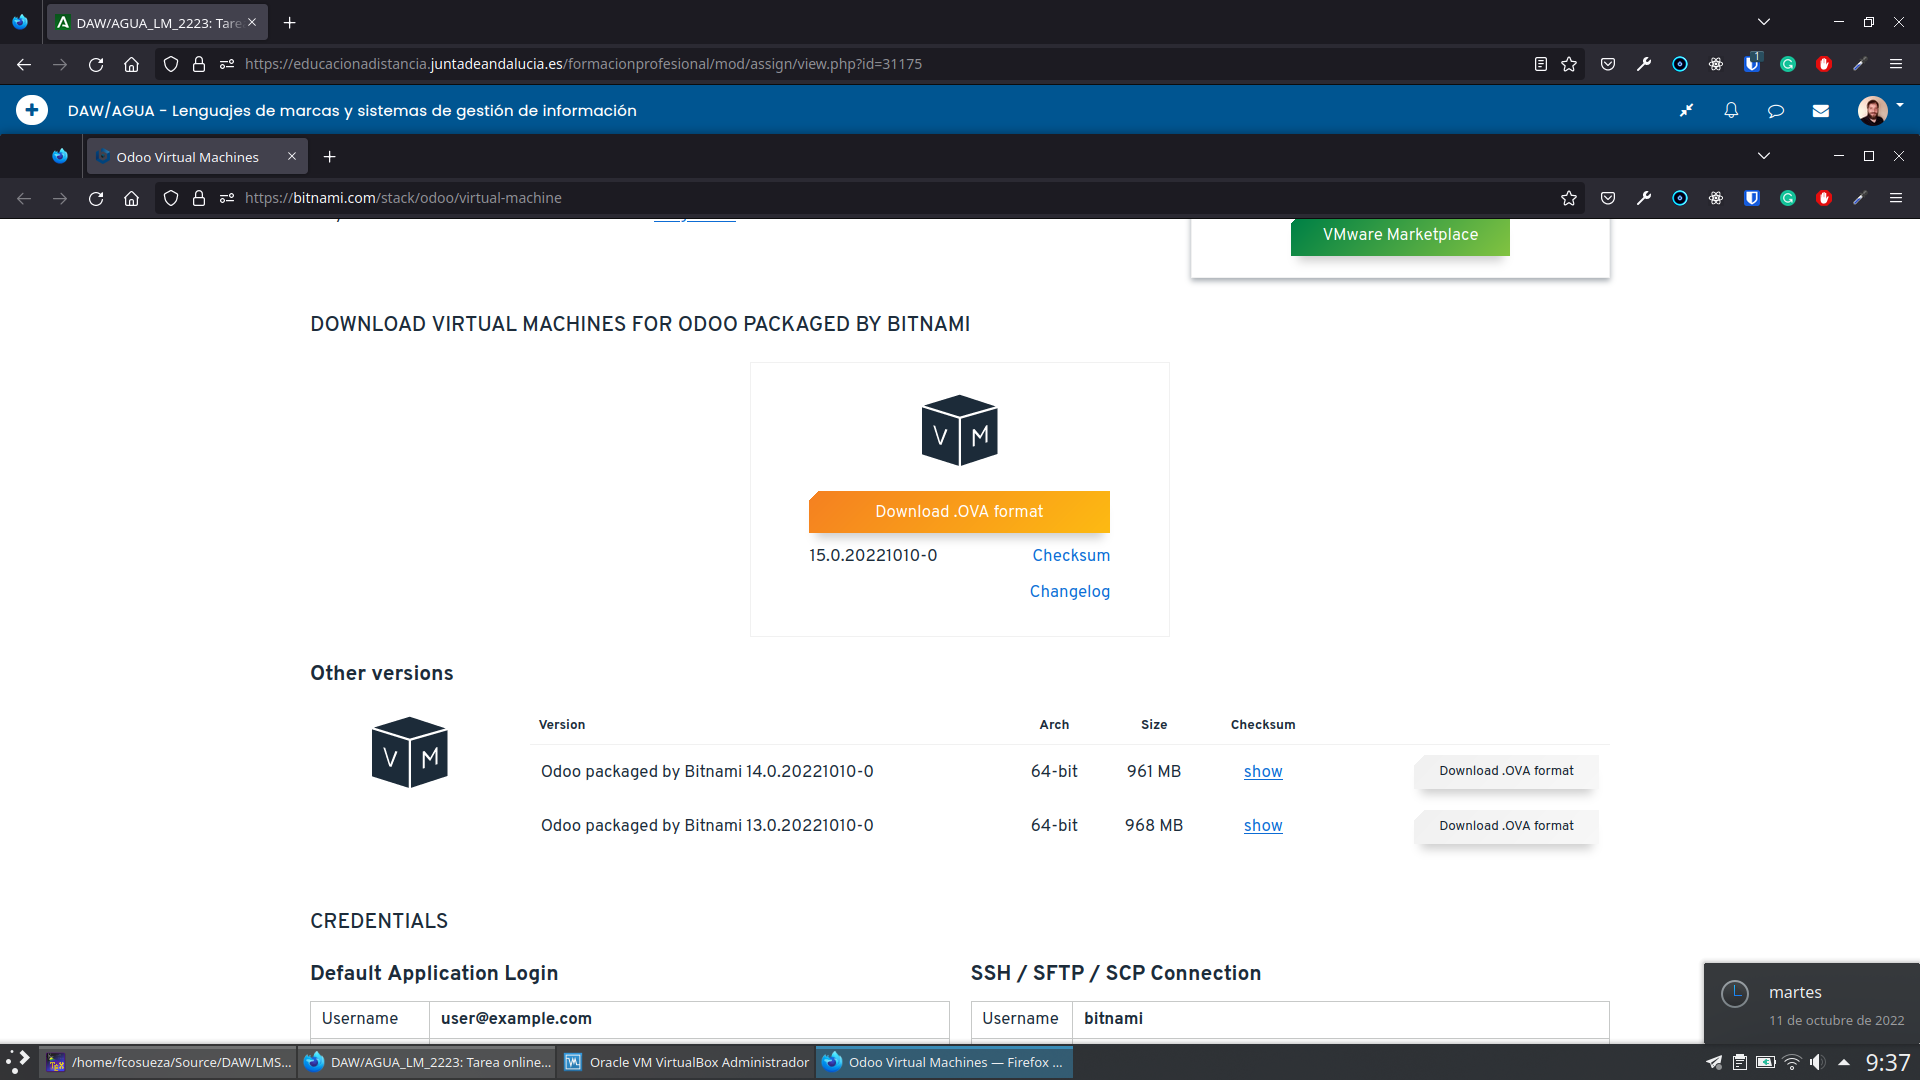
\includegraphics[scale=0.25]{descarga-odoo.png}
    \caption{Página de Bitnami con la imagen de Odoo}
\end{figure}


\subsection{Instalación de la imagen en VirtualBox}
Una vez que tengamos descargada la imagen, ya podemos proceder a su instalación en VirtualBox. Para ello abrimos la aplicación y seleccionamos la opción \textit{\textbf{Import}} como se muestra en la siguiente captura.

\begin{figure}[h]
    \centering
    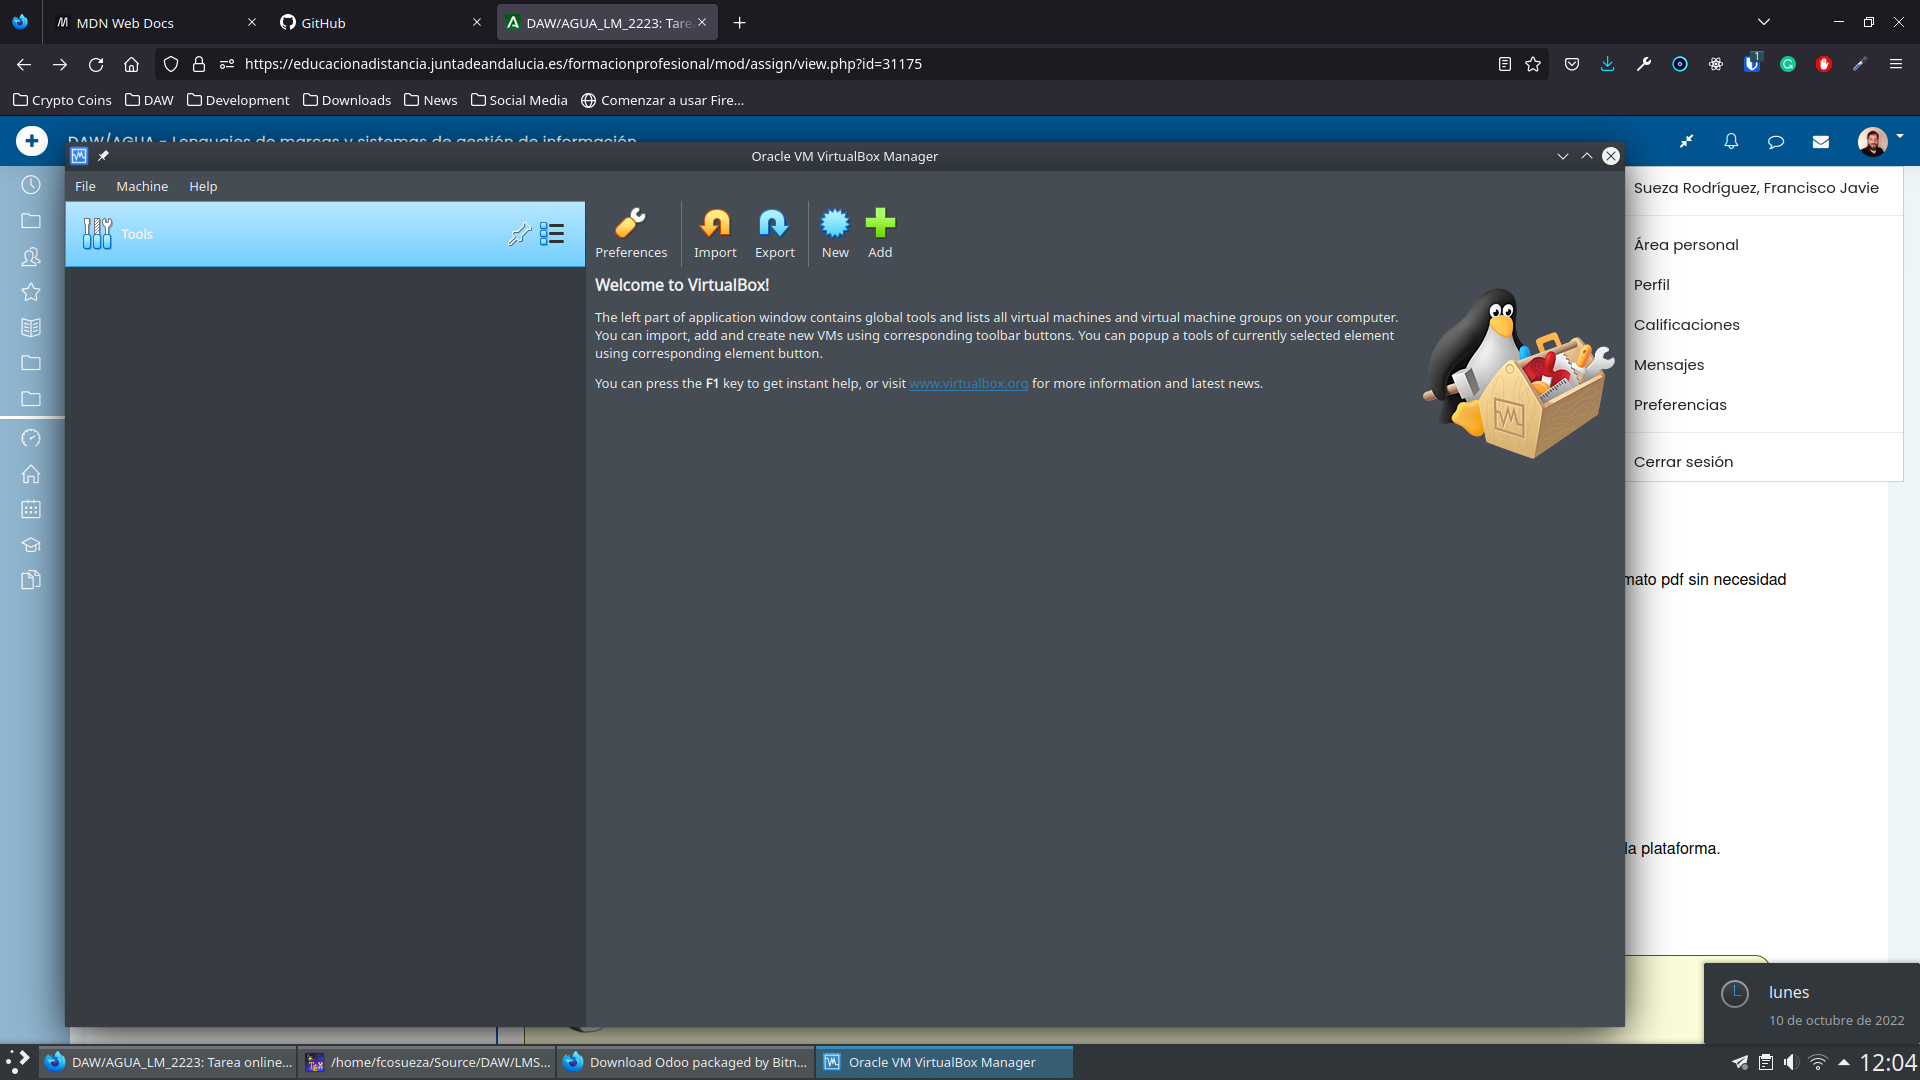
\includegraphics[scale=0.25]{vb-import.png}
    \caption{Pantalla principal de VirtualBox}
\end{figure}

A continuación, cargamos la imagen que nos acabamos de descargar, y pulsamos en Next para continuar con el proceso de instalación. Deberemos seleccionar la imagen que tenemos descargada en nuestro disco duro y continuar. Se nos mostrará una página con la información de la imagen de Odoo y tras pulsar de nuevo en \textbf{\textit{Import}}, nuestra imagen quedará carga en la máquina virtual.

\begin{figure}[h]
    \centering
    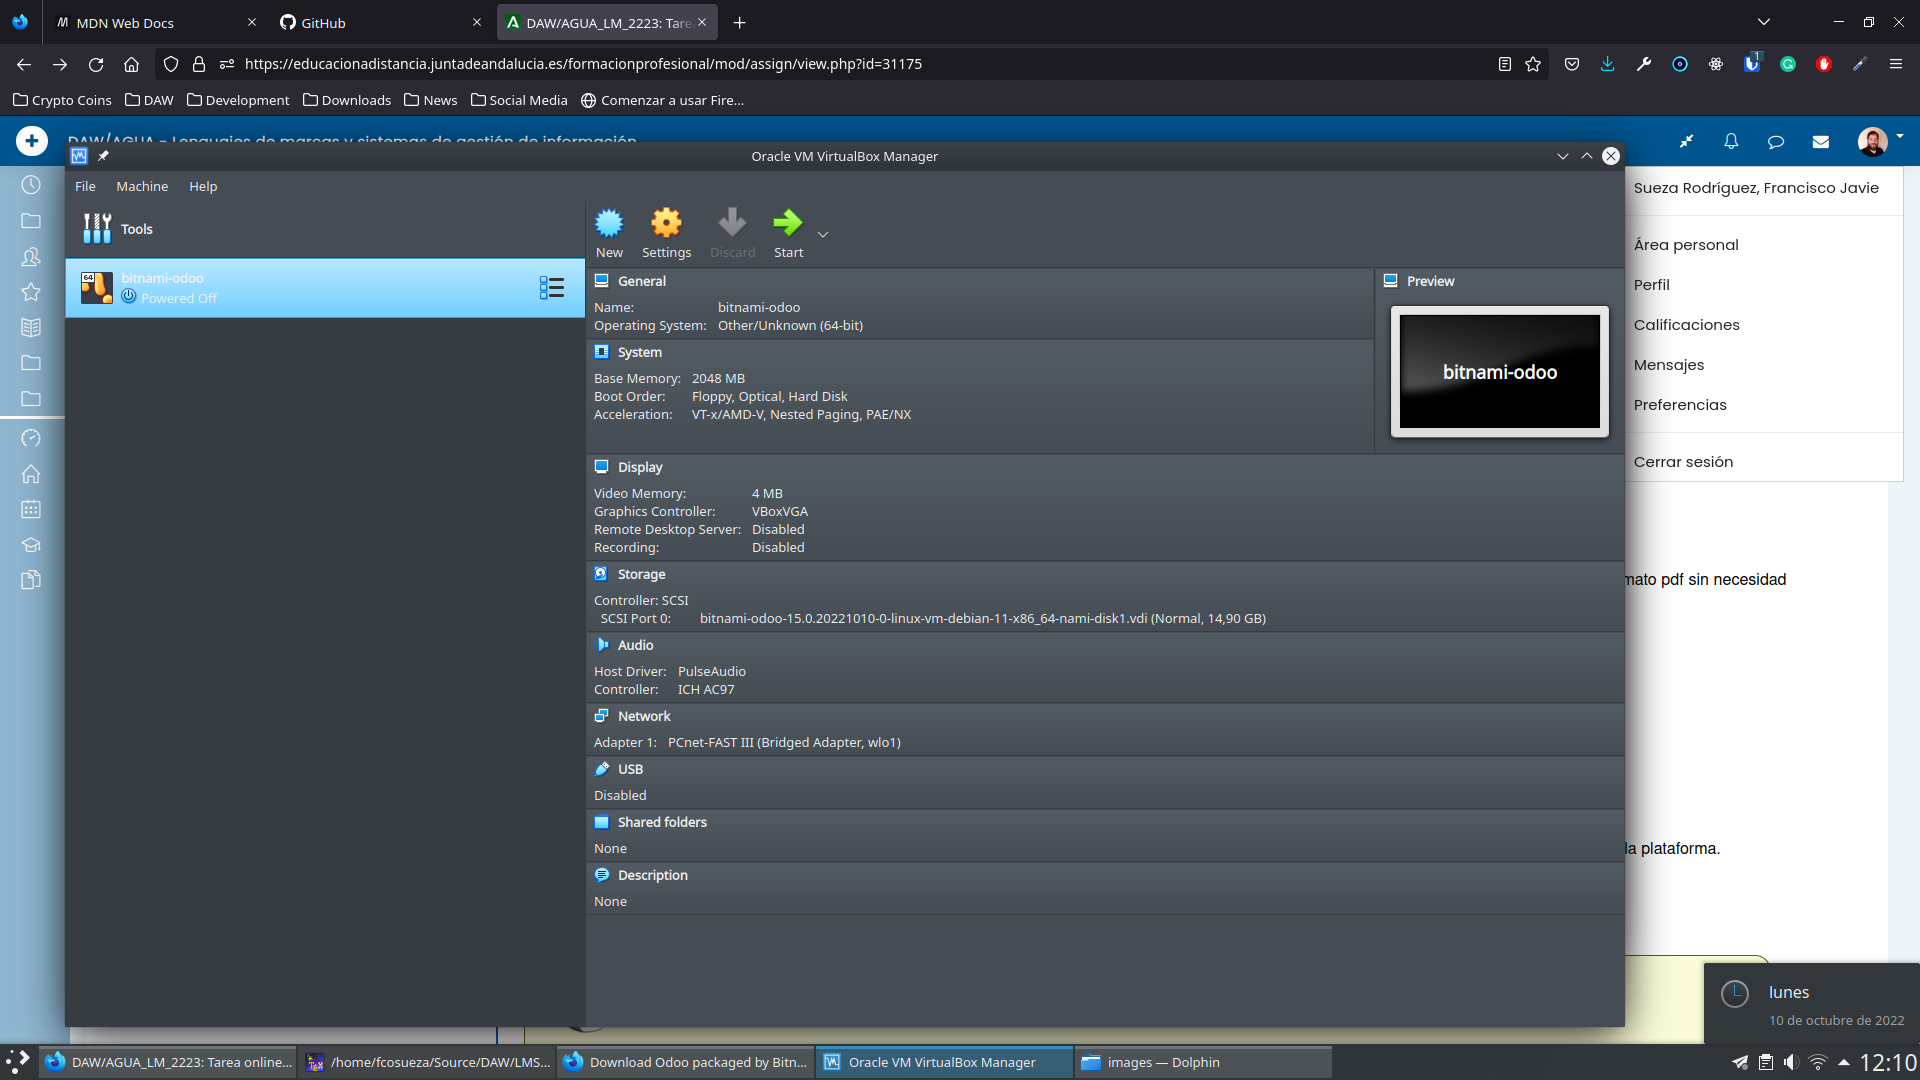
\includegraphics[scale=0.25]{vb-image-loaded.png}
    \caption{Imagen de Odoo cargada en VirtualBox}
\end{figure}

Después de esto, ya tendremos la imagen lista para usar en VirtualBox y podremos comenzar a utilizar Odoo. Cabe destacar que esta imagen ya trae Odoo instalado y configurado, ya que esta pensado para probar el sistema y ver si se adapta a nuestra necesidades. Si realizáramos una instalación local, requeriríamos más pasos, como la instalación de paquetes de de bases de datos y demás. Podemos encontrar más información sobre los diferentes tipos de instalaciones en la \href{https://www.odoo.com/documentation/15.0/administration/install/install.html}{Documentación oficial de Odoo}.

\subsection{Accediendo a Odoo}
Una vez que tenemos la imagen cargada en VB, deberemos inicial, para lo que pulsaremos el botón \textbf{\textbf{Start}} o haremos doble click sobre la imagen de Odoo que se nos muestra en la lista de la izquierda. Esto iniciara una nueva ventana donde se nos mostrará información muy útil sobre la instalación y la máquina virtual.

\begin{figure}[h]
    \centering
    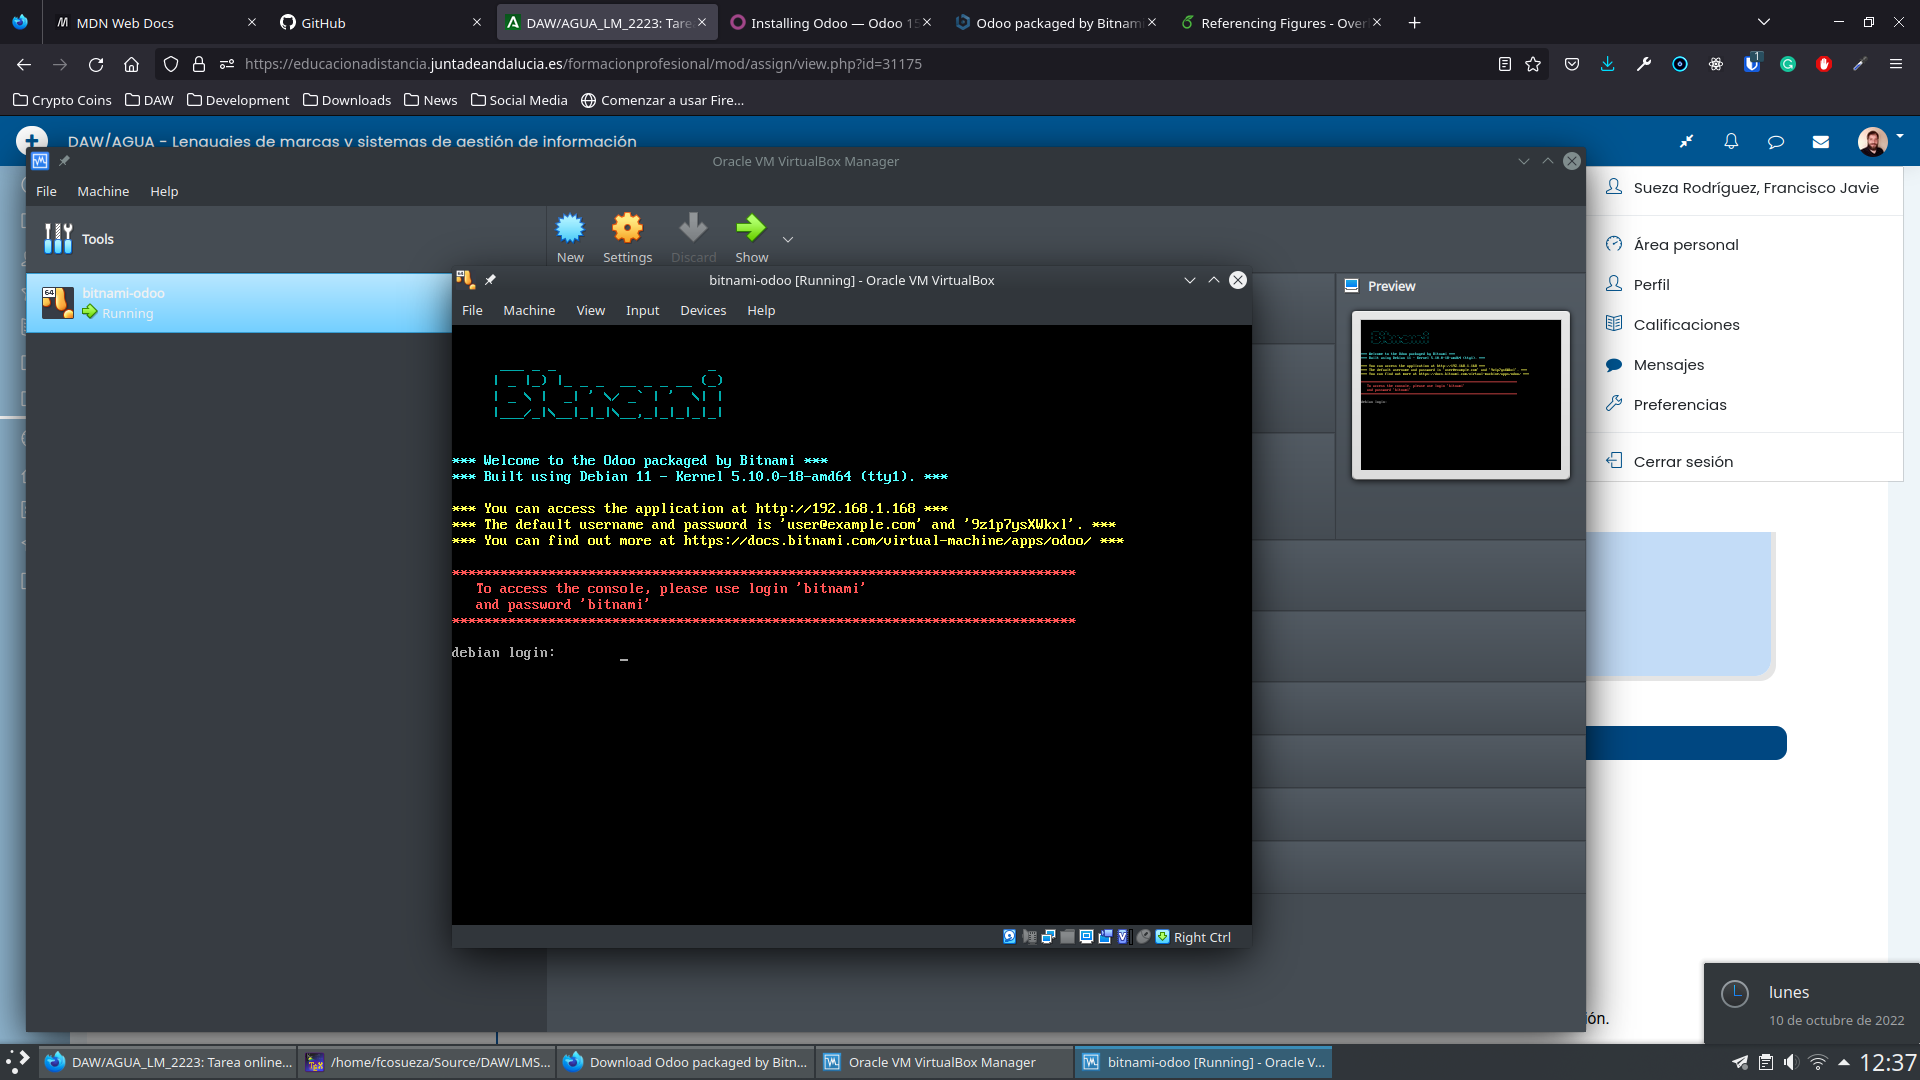
\includegraphics[scale=0.25]{vb-image-main.png}
    \caption{Pantalla principal de la imagen Odoo en VB}
\end{figure}

En esta pantalla se nos muestra diferente información que nos va a ser útil. La más importante es la\textbf{ dirección web} del servidor, en este caso es \textbf{\textit{http://192.168.1.168}}, con la que podremos acceder a Odoo desde un navegador instalado en nuestro PC. Y por otro lado, nos muestra los \textbf{credenciales por defecto} de Odoo, en este caso son \textbf{usuario}: \textit{user@example.com} y \textbf{contraseña}: \textit{9z1p7ysXWkxl}. Además de esta información se nos muestra el usuario y contraseña del sistema operativo, aunque ahora mismo no lo necesitamos para nada.

Con esta información, vamos a abrir un navegado, introducir la dirección web facilitada y los credenciales, para así poder acceder a Odoo.

% Bibliography

\newpage
\bibliography{citas}
\bibliographystyle{unsrt}

\end{document}